
\section{Deliverable 2: Linear separable dataset}


\begin{solve}    

\begin{figure}[H]
    \centering
    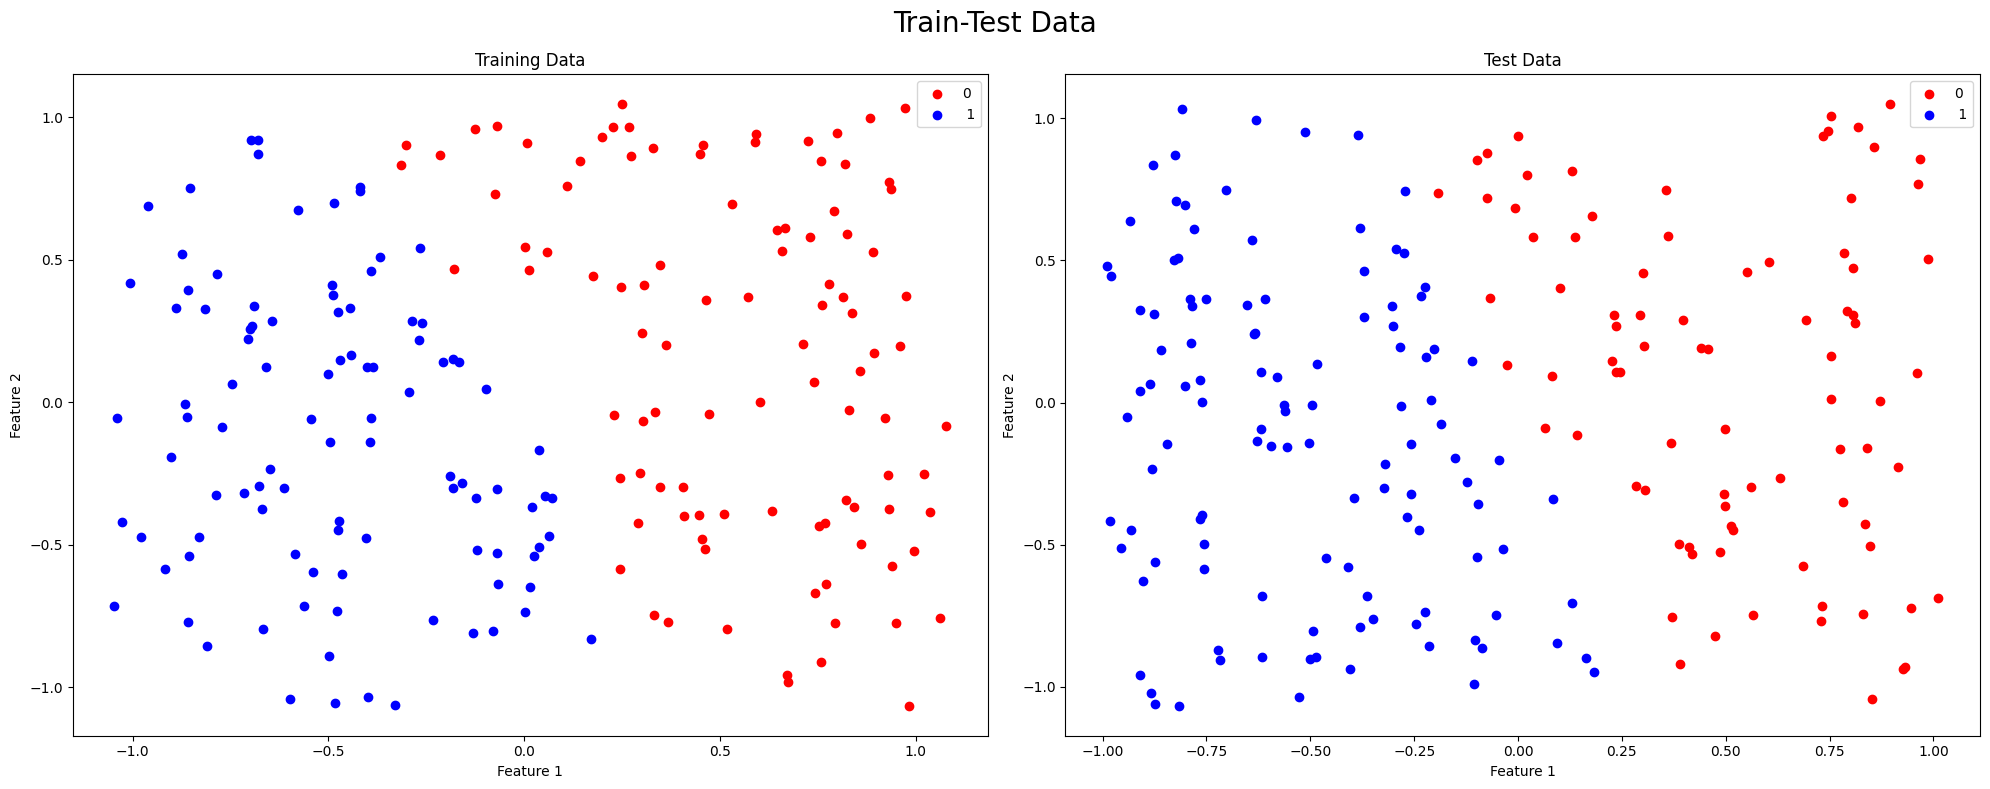
\includegraphics[width=0.7\textwidth]{plots/2_lineardataset.png}
    \caption{Linear separable dataset (train, test set with 200 points each)}
\end{figure}

\begin{lstlisting}[language=python]

dim_in, dim_out = x_train.shape[1], 2
hidden_neuron_list = [1]
activation_list = ['ReLU', 'Sigmoid']
opt_init = None
opt_loss = L2Loss()
mlp = MLP(dim_in, dim_out, hidden_neuron_list, activation_list, opt_init)
opt_optim = SGD(mlp)
----------------------------------------

Model Summary
-------------
Layer 1: Linear - A Dim: 2, Output Dim: 1, Parameters: 3
Layer 2: ReLU
Layer 3: Linear - A Dim: 1, Output Dim: 2, Parameters: 4
Layer 4: Sigmoid
Total Parameters: 7
\end{lstlisting}

\begin{figure}[H]
    \centering
    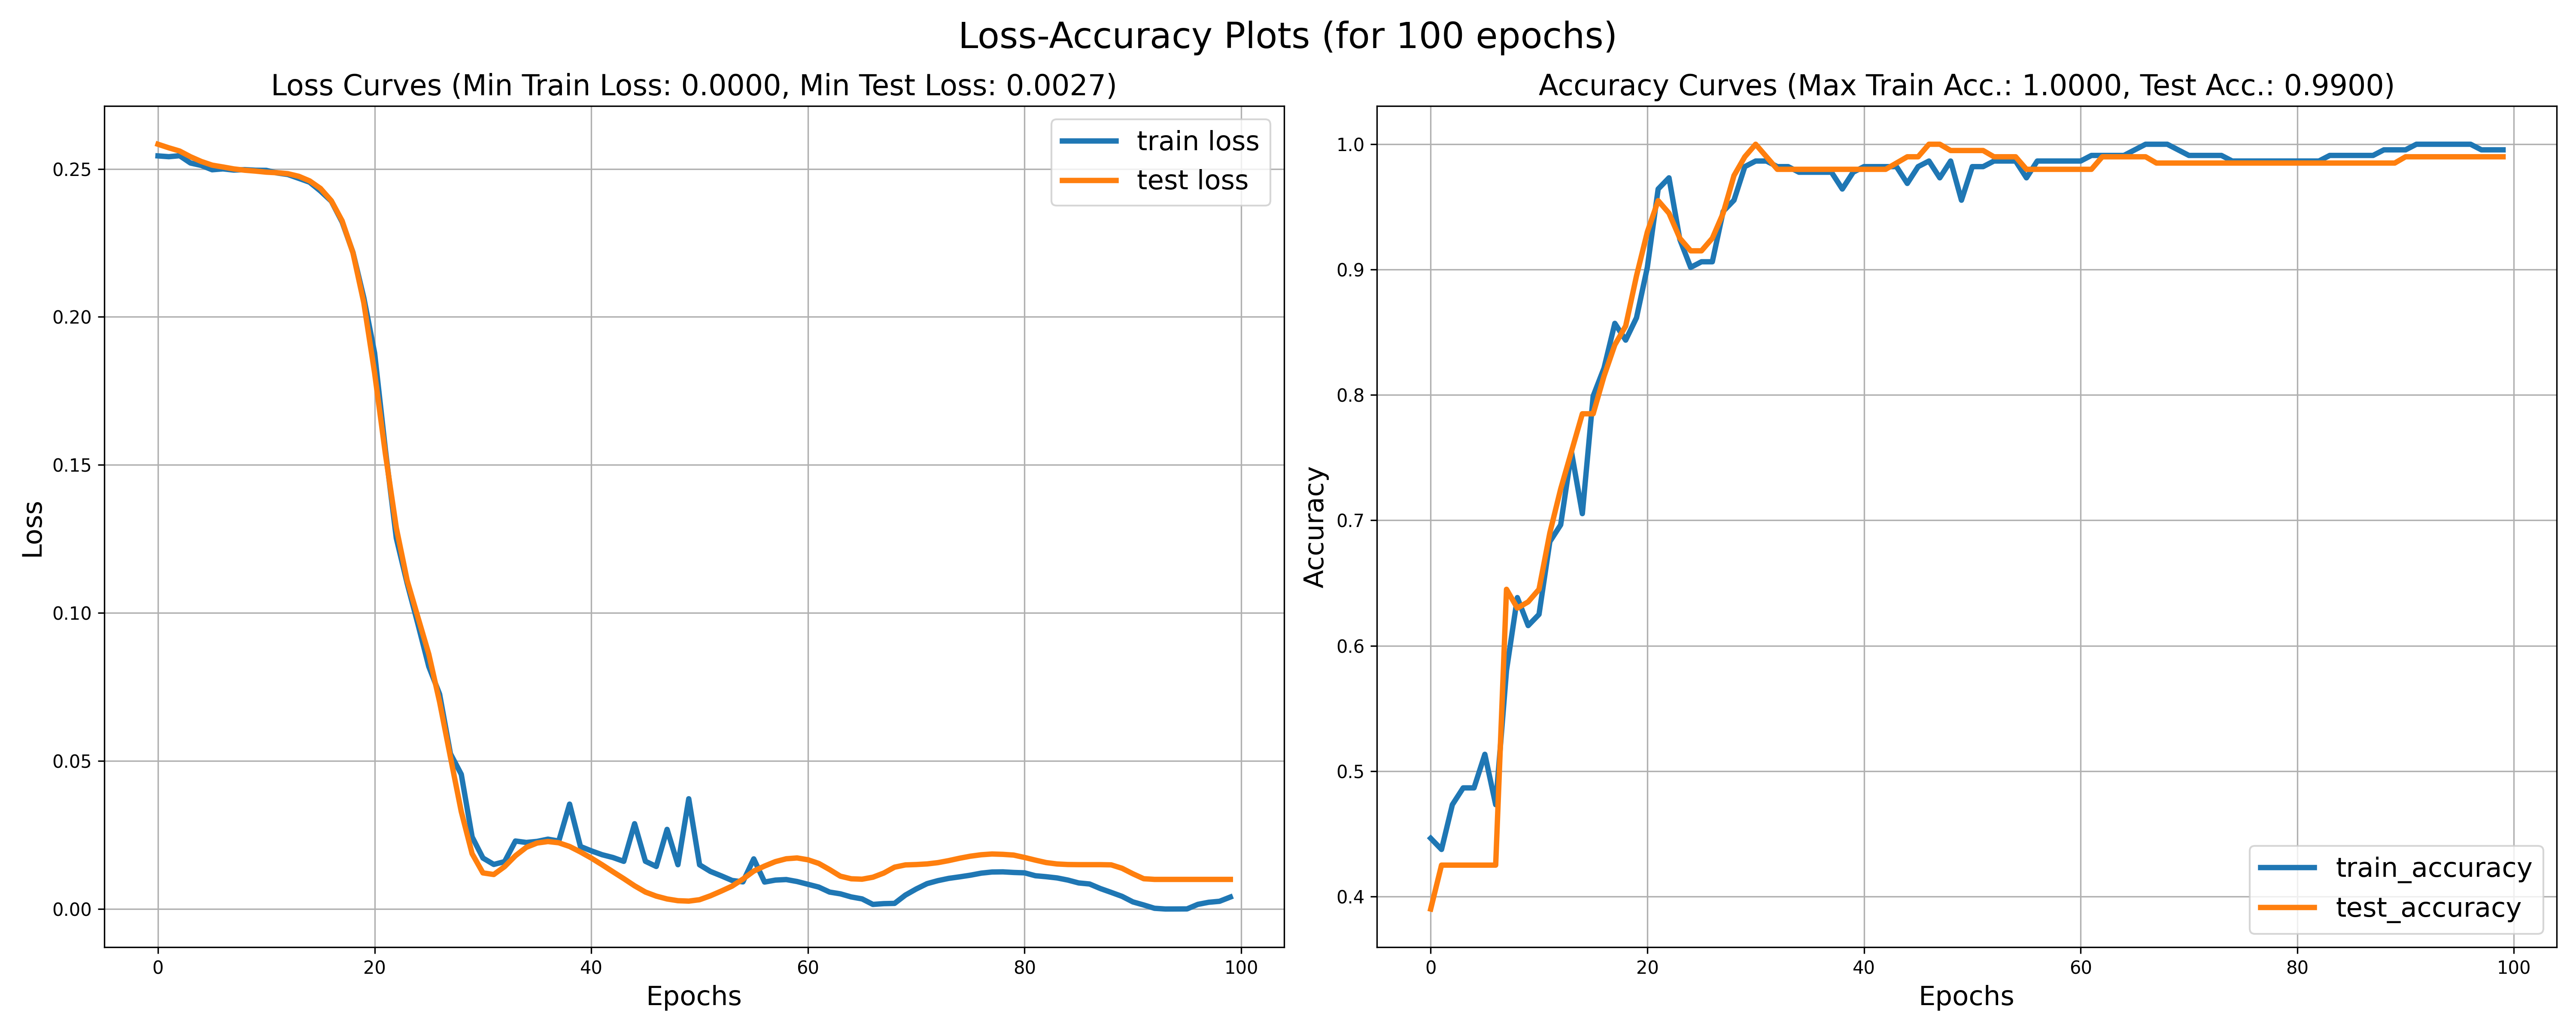
\includegraphics[width=0.8\textwidth]{plots/2_linearloss_acc.png}
    \caption{Loss and accuracy for linear separable dataset (train, test set with 200 points each)}
\end{figure}

\begin{figure}[H]
    \centering
    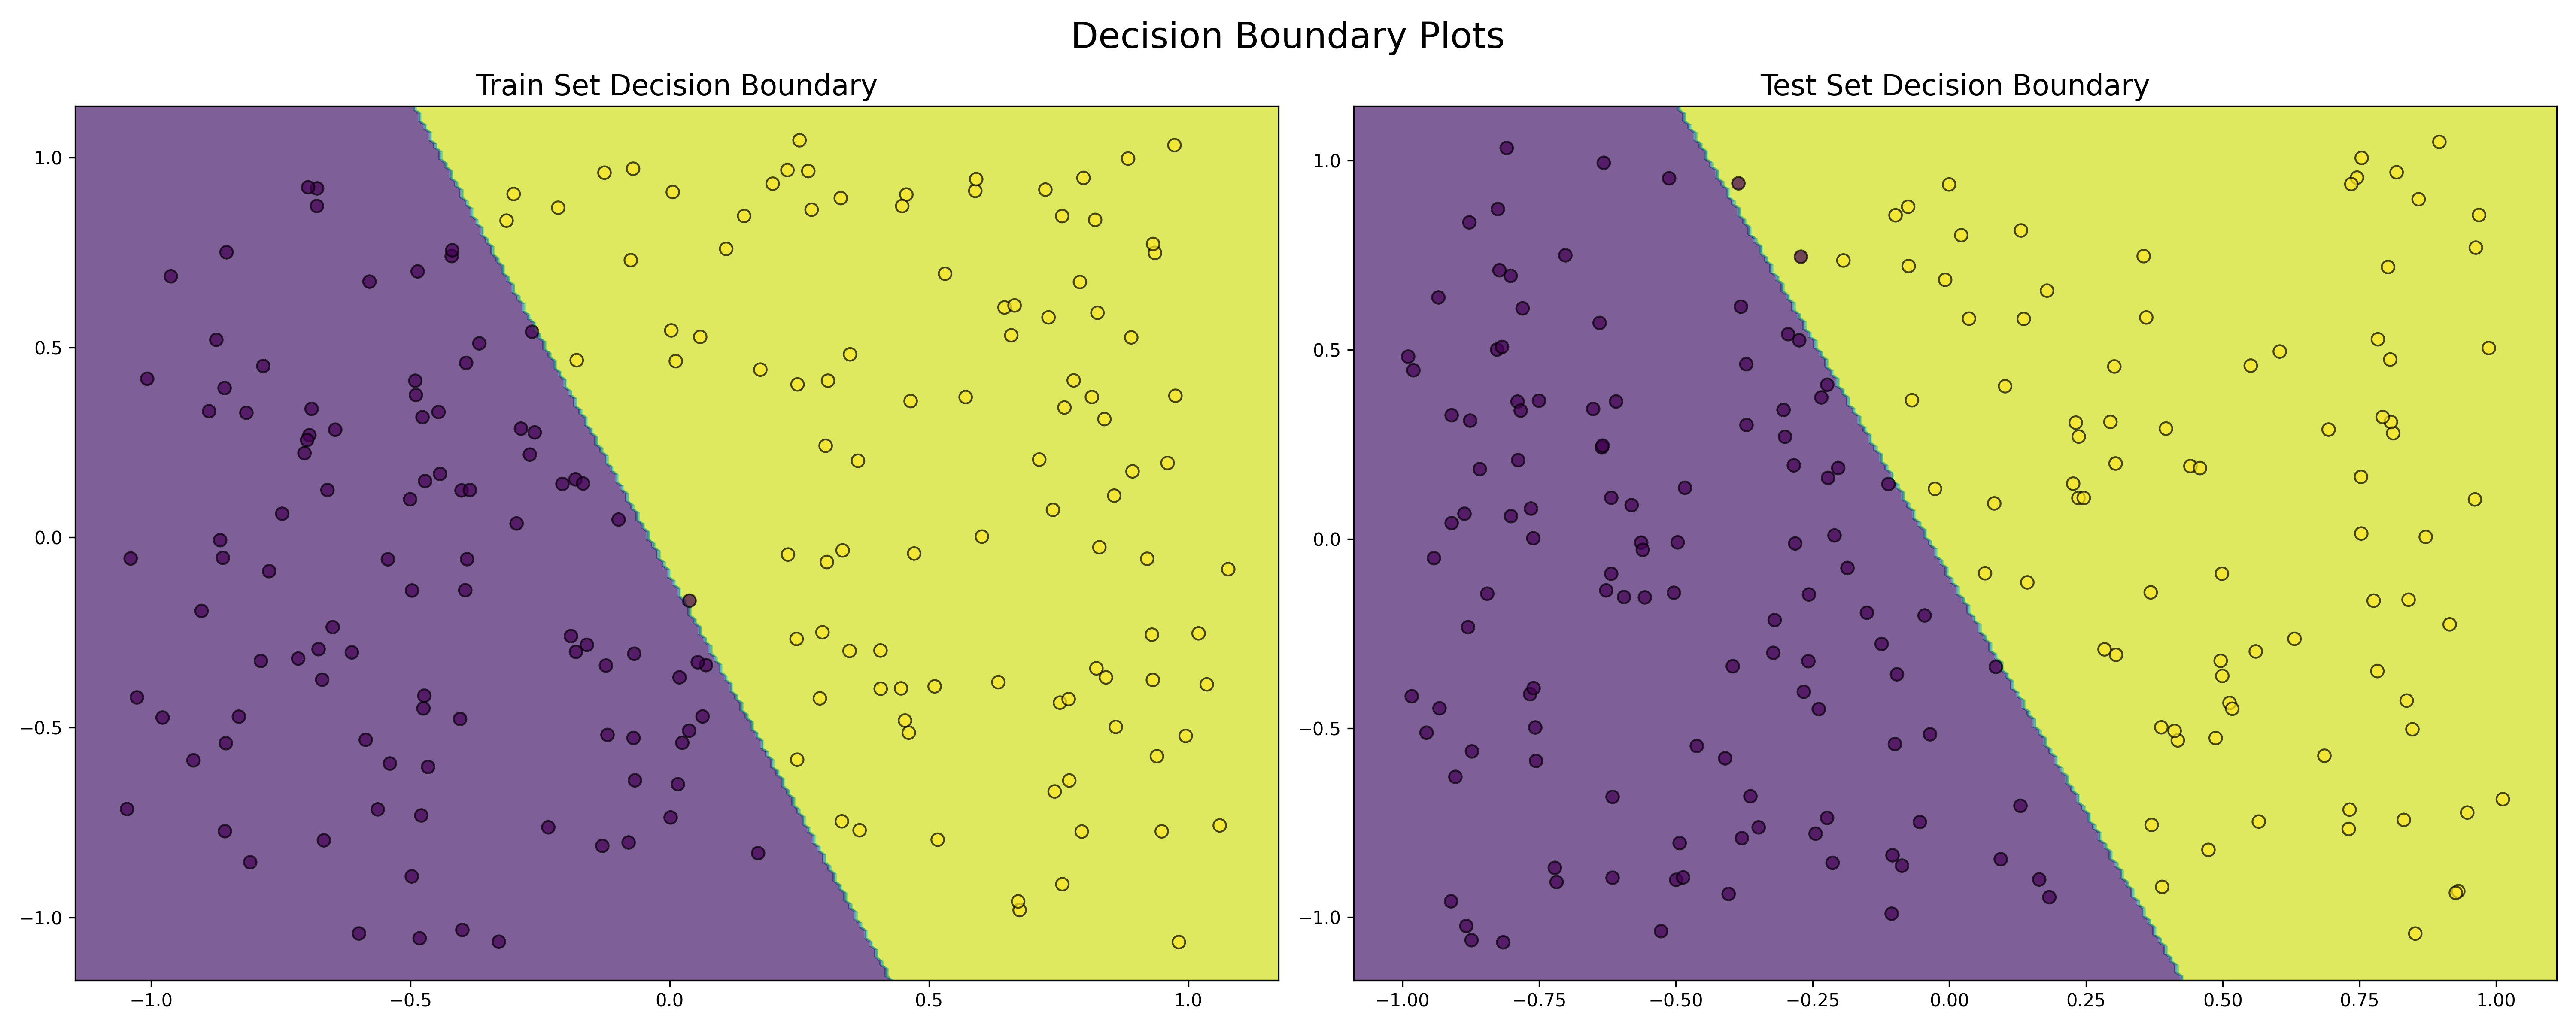
\includegraphics[width=0.7\textwidth]{plots/2_linearboundary.png}
    \caption{Decision boundary for linear separable dataset (train, test set with 200 points each)}
\end{figure}

\end{solve}
